%=========================
\chapter{La récursivité}
%=========================

\begin{center}
	{\itshape «~Pour comprendre le principe de récursivité, 
	
	il faut d'abord comprendre le principe de récursivité~»}

	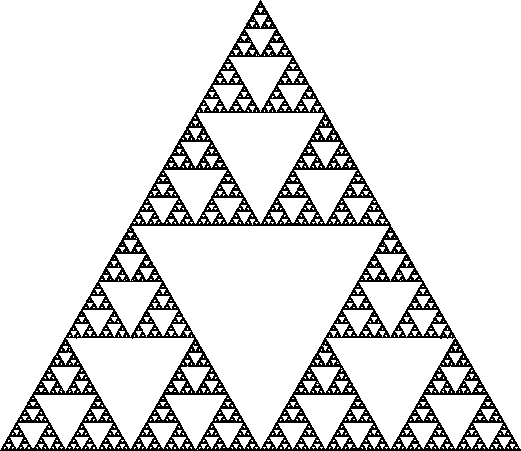
\includegraphics[width=4.094cm,height=3.519cm]{image/a2012Logique2eme-img015.png}
\end{center}
	

%=====================
\section{Introduction}
%=====================
	
	Une procédure est dite \textbf{récursive} lorsque dans sa description, 
	une des étapes de cette procédure est la procédure elle-même. 
	Des termes synonymes de la récursivité sont la \textbf{récurrence} 
	ou l'\textbf{auto-référence}.
	
	\textit{La récursivité est une démarche qui consiste à faire 
	référence à ce qui fait l'objet de la démarche, ainsi c'est
	le fait de décrire un processus dépendant de données en faisant 
	appel à ce même processus sur d'autres données plus
	«simples», de montrer une image contenant des images similaires, 
	de définir un concept en invoquant le même concept.
	(Wikipédia, août 2013)}

	Les illustrations ci-dessous sont des exemples célèbres 
	de dessins récursifs~:

	{
	 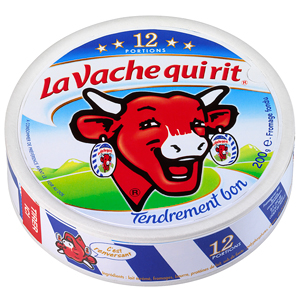
\includegraphics[width=5.41cm,height=5.41cm]{image/a2012Logique2eme-img016.jpg} 
	\ \ \ \ \ \ \ \ \ 
	\href{http://upload.wikimedia.org/wikipedia/commons/6/62/Droste.jpg}{
	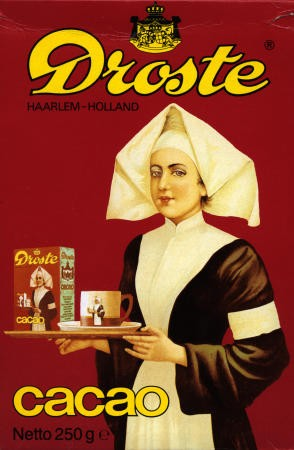
\includegraphics[width=3.328cm,height=5.098cm]{image/a2012Logique2eme-img017.jpg} } 
	\ \ \ \ \ \ \ \ \ 
	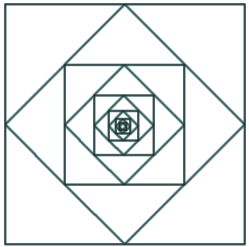
\includegraphics[width=5.089cm,height=5.052cm]{image/a2012Logique2eme-img018.png} }


	La \textit{vache qui rit} qui orne la fameuse boite 
	de fromage porte des boucles d'oreilles en forme de boites de
	fromage identiques au dessin entier. Il en est de même pour 
	le dessin de la boite de cacao \textit{Droste}~: sur le
	plateau porté par la dame apparait en plus petit la même 
	boite de cacao. Dans le troisième dessin, chaque carré
	contient un carré plus petit inscrit dans le carré précédent 
	de telle sorte que l'image formée à partir du 3\textsuperscript{e} 
	carré est identique au carré de départ, mais réduite de 50\%. 
	Chacun de ces dessins s'\textit{auto-contient} donc à une échelle 
	plus petite. Il en est de même pour le dessin fractal en haut de
	ce chapitre, il s'agit du \textit{triangle de Sierpinski} 
	formé dans chaque coin de triangles plus petits mais pareils
	au triangle entier.


%===============================
\section{Définitions récursives}
%===============================

	Les dessins ci-dessus offrent des exemples de \textit{récursivité infinie}. 
	En mathématique et en informatique, la récursivité définit plutôt un 
	processus dont la description se décompose en un (ou plusieurs) cas de base, 
	et un	ensemble de régles réduisant les autres cas aux cas de base 
	par l'exécution d'un nombre fini d'étapes.

	Certains concepts peuvent se définir récursivement, 
	à condition que la définition contienne une clause d'évaluation
	immédiate sans appel récursif. Prenons par exemple la formule 
	\textit{récursive} de la factorielle~: 
	$n! = n*(n-1)!$

	Cette formule est incomplète si on ne définit pas le cas initial 
	$0! = 1$. À partir du cas de base et de la formule
	récursive, on peut calculer la factorielle de n'importe quel entier.

	Parmi les autres exemples rencontrés au cours de mathématique, 
	citons la formule récursive des coefficients binomiaux~:


	{\centering
	 $C_n^p=C_{n-1}^{p-1}+C_{n-1}^p$\ \ si $0<p<n$
	\par}

	avec les cas de bases~: $C_n^0=1$ et $C_n^n=1$. 
	
	Cette définition permet de reconstruire facilement le triangle de Pascal~:

	\begin{center}
	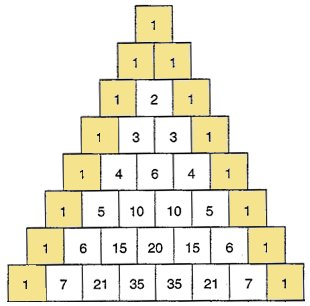
\includegraphics[width=4.724cm,height=4.651cm]{image/a2012Logique2eme-img019.jpg}
	\end{center}

	Noter que le calcul récursif est plus commode d'utilisation 
	que la formule «~directe~»~faisant intervenir les
	factorielles~:

	{\centering
	$C_n^p=\frac{n!}{(n-p)!p!}$
	\par}
	
	Un troisième exemple est la formule récursive pour 
	calculer les nombres de Fibonacci~:
	
	{\centering
	$F_n=F_{n-1}+F_{n-2}$
	\par}
	
	avec les cas initiaux $F_0 = 1$ et $F_1 = 1$. 
	
	Cette formule récursive est bien plus maniable la formule 
	donnant «~directement~» le \textit{n}\textsuperscript{ième} 
	nombre de Fibonacci~:
	
	{\centering
	$F_n=\frac{1}{\sqrt{5}} * (\frac{1+\sqrt{5}}{2})^n - \frac{1}{\sqrt{5}} * (\frac{1-\sqrt{5}}{2})^n $
	\par}

	On peut aussi définir de façon récursive certaines structures 
	courantes en informatique, comme le montre par
	exemple cette définition récursive de la liste chainée~:

	\textit{
	une liste chainée est un ensemble soit vide, 
	soit composé d'un élément auquel est attaché une liste chainée.}

	Cette définition est intelligible par le fait qu'on sous-entend 
	que la liste chainée à laquelle la définition fait
	référence n'est plus identique à la première, mais plus 
	petite d'un élément, et éventuellement qu'elle peut se terminer
	(ensemble vide).

	On peut de façon semblable définir une chaine de caractères~:

	\textit{une chaine de caractères est un ensemble soit vide, 
	soit composé d'un caractère concaténé à une chaine de caractères.}
	

%============================
\section{Algorithme récursif}
%============================

	En informatique, un \textbf{algorithme récursif} est 
	un algorithme qui, lors de son exécution, fait appel une ou
	plusieurs fois à lui-même. Ainsi, dans un module récursif, 
	nous pourrons écrire parmi les instructions l'appel à ce
	module lui-même~:

	\cadre{
		\begin{pseudo}
			\Module{récursif}{...}{}
				\LComment instructions
				\Stmt récursif(...)
				\LComment instructions
			\EndModule
		\end{pseudo}
	}

	Si cette situation peut surprendre au premier abord, elle 
	n'est pourtant pas très différente de la situation suivante,
	appelée \textit{récursivité croisée~}:

	\cadre{
		\begin{pseudo}
			\Module{premier}{...}{}
				\LComment instructions
				\Stmt second(...)
				\LComment instructions
			\EndModule
		\end{pseudo}
	}
	
	\cadre{
		\begin{pseudo}
			\Module{second}{...}{}
				\LComment instructions
				\Stmt premier(...)
				\LComment instructions
			\EndModule
		\end{pseudo}
	}

	Chaque module fait appel à l'autre, et si on recopie le code 
	du module second à la place de son appel dans premier, on
	obtient la même situation que dans le module récursif qui 
	précède. Néanmoins, en absence de paramètres, ces deux
	situations génèrent un processus infini, et pire, une 
	saturation de la mémoire ! En effet, pour pouvoir fonctionner,
	chaque appel du module génère un nouvel ensemble des variables 
	utilisées dans le module. La situation est donc très
	différente d'une boucle infinie du type \textit{tant que} 
	ou \textit{faire jusqu'à ce que}.

	Pour ne pas tomber dans ce processus sans fond, un algorithme 
	récursif bien écrit doit forcément posséder un (ou plusieurs) 
	paramètre(s), et contenir une structure alternative qui conduit 
	à une clause d'évaluation immédiate  appel récursif pour une 
	(ou plusieurs) valeur(s) initiale(s) des paramètre(s). 
	La forme générale est la suivante~:

	\cadre{
		\begin{pseudo}
			\Module{récursif}{paramètre}{}
				\If{paramètre = valeur initiale}
					\LComment il peut y avoir plusieurs cas initiaux
					\LComment instructions sans appel récursif.
				\Else
					\LComment instructions menant à des valeurs différentes du paramètre, 
					\LComment et après un nombre fini d'appels récursifs aux valeurs initiales.
				\EndIf
			\EndModule
		\end{pseudo}
	}

%============================
\section{Exemples classiques}
%============================

	Dans ce paragraphe, nous présentons quelques grands 
	classiques de la programmation récursive.


	\subsection{La factorielle}
	%==========================

		Le module récursif calculant la factorielle d'un entier positif 
		est issu directement de la définition récursive rappelée
		ci-dessus~:

		\cadre{
			\begin{pseudo}
				\Module{factorielle}{n\In~: entier}{entier}
					\If{n = 0}
						\Return 1
					\Else
						\Return $n*factorielle(n - 1)$
					\EndIf
				\EndModule
			\end{pseudo}
		}

		Comment cela fonctionne-t-il ? Par exemple, si le module est 
		appelé avec la valeur 3 du paramètre, il doit calculer 3 fois la 
		factorielle de 2. Le calcul est donc mis en attente jusqu'à ce 
		que la factorielle de 2 soit connue ; et il en est de même pour 
		le calcul de factorielle de 2, qui appelle la factorielle de 1 
		qui à son tour appelle la factorielle de 0. À ce moment, la 
		valeur 1 est retournée, et les renvois se font en cascade 
		jusqu'au premier appel qui peut enfin retourner la valeur 6.

		\begin{center}
		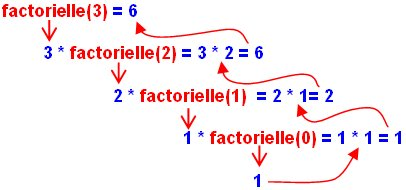
\includegraphics[width=8.902cm,height=4.159cm]{image/a2012Logique2eme-img021.jpg}
		\end{center}

	\subsection{Les tours de Hanoï}
	%==============================

		Il s'agit d'un jeu de réflexion consistant à déplacer une tour formée 
		de \textit{n} disques de diamètres différents. La tour qui se trouve 
		sur un socle de départ doit être reconstruite sur un socle d'arrivée, 
		en utilisant un socle intermédiaire, en en respectant les règles suivantes~:

		\begin{itemize}
			\item {
				on ne peut déplacer qu'un disque à la fois}
			\item {
				on ne peut jamais placer un disque sur un autre disque de diamètre plus grand}
		\end{itemize}

		\begin{center}
		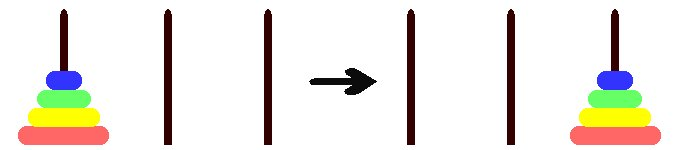
\includegraphics[width=14.002cm,height=3cm]{image/a2012Logique2eme-img022.jpg}
		\end{center}

		On voudrait écrire un algorithme qui affiche la liste des déplacements 
		des disques qui conduisent à la reconstruction de la tour. La récursivité 
		permet de décrire très simplement la marche à suivre~: supposons qu'on 
		sache comment reconstituer une tour de \textit{n--1} disques, la 
		reconstitution d'une tour de \textit{n} disques est alors un jeu d'enfant 
		et s'exécute en 3 étapes~:

		\begin{itemize}
			\item {
				reconstituer la tour formée par les \textit{n - 1} disques les plus 
				petits du socle de départ vers le socle intermédiaire (en utilisant 
				le socle d'arrivée comme socle intermédiaire)}
				
				\begin{center}
				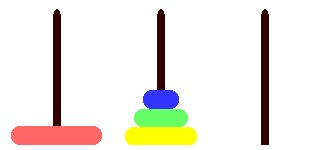
\includegraphics[width=6.692cm,height=2.99cm]{image/a2012Logique2eme-img023.jpg}
				\end{center}
				
			\item {
				déplacer le disque le plus grand du socle de départ vers le socle d'arrivée}
				\begin{center}
				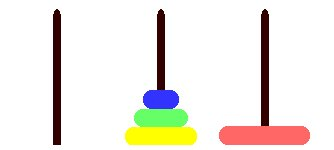
\includegraphics[width=6.668cm,height=3cm]{image/a2012Logique2eme-img024.jpg}
				\end{center}
			
			\item {
				reconstituer la tour formée par les \textit{n -- 1} disques les plus 
				petits du socle intermédiaire vers le socle d'arrivée (en utilisant 
				cette fois-ci le socle de départ comme socle intermédiaire)}
			\begin{center}
			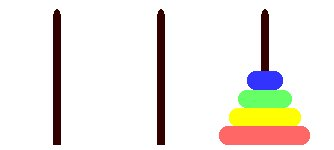
\includegraphics[width=6.703cm,height=3cm]{image/a2012Logique2eme-img025.jpg}
			\end{center}
		\end{itemize}
		
		Cette démarche conduit au code suivant~(les socles sont déclarés comme
		caractères, on peut leur donner des noms 'A', 'B' et 'C'par exemple)~:

		\cadre{
			\begin{pseudo}
				\Module{Hanoï}{n\In~: entier, départ\In, arrivée\In, intermédiaire\In~:
		caractères)}{}
					\If{n > 0}
						\Stmt Hanoï(n -- 1, départ, intermédiaire, arrivée)
						\Write «~déplacer le disque de taille~», n «~du socle~», départ, «~vers le socle~»,	arrivée
						\Stmt Hanoï(n -- 1, intermédiaire, arrivée, départ)
					\EndIf
				\EndModule
			\end{pseudo}
		}

	\subsection{Le tri Quicksort}
	%============================
	
		Il s'agit -- comme son nom l'indique -- d'une technique de 
		\textit{tri rapide} des éléments d'un tableau. L'idée est
		relativement simple~: on choisit d'abord un élément pivot 
		(aléatoirement ou de façon déterminée ; en pratique, c'est
		l'élément du milieu). On réarrange ensuite -- par un nombre 
		minimum de déplacements -- le tableau de façon à le partager 
		en deux sous-tableaux~: à gauche les éléments inférieurs au 
		pivot, et à droite les éléments supérieurs au pivot. Il suffit 
		ensuite de réappliquer l'algorithme de façon récursive à chacun 
		des sous-tableaux obtenus. Lorsque la taille d'un sous-tableau 
		est inférieure à 2, il n'y a alors plus rien à trier.

		Montrons le fonctionnement de l'algorithme sur un exemple. 
		Pour le tableau suivant, le pivot sera le 5\textsuperscript{e} 
		élément, de valeur 6~

		\begin{center}
			\tablefirsthead{}
			\tablehead{}
			\tabletail{}
			\tablelasttail{}
			\begin{supertabular}{|m{1.171cm}|m{1.206cm}|m{1.206cm}|m{1.206cm}|m{1.206cm}|m{1.206cm}|m{1.206cm}|m{1.206cm}|m{1.206cm}|m{1.232cm}|}
			\hline
			\centering{\sffamily 4} &
			\centering{\sffamily 3} &
			\centering{\sffamily 8} &
			\centering{\sffamily 9} &
			\centering{\sffamily \cellcolor{gray!25}6} &
			\centering{\sffamily 3} &
			\centering{\sffamily 7} &
			\centering{\sffamily 1} &
			\centering{\sffamily 5} &
			\centering\arraybslash{\sffamily 3}\\\hline
			\end{supertabular}
		\end{center}

		Le réarrangement se fait en échangeant le premier élément supérieur 
		ou égal au pivot (en partant de la gauche) avec le premier élément 
		inférieur ou égal au pivot (en partant de la droite)~:

		\begin{center}
			\tablefirsthead{}
			\tablehead{}
			\tabletail{}
			\tablelasttail{}
			\begin{supertabular}{|m{1.171cm}|m{1.206cm}|m{1.206cm}|m{1.206cm}|m{1.206cm}|m{1.206cm}|m{1.206cm}|m{1.206cm}|m{1.206cm}|m{1.232cm}|}
			\hline
			\centering{\sffamily 4} &
			\centering{\sffamily 3} &
			\centering{\sffamily \cellcolor{gray!25}8} &
			\centering{\sffamily 9} &
			\centering{\sffamily 6} &
			\centering{\sffamily 3} &
			\centering{\sffamily 7} &
			\centering{\sffamily 1} &
			\centering{\sffamily 5} &
			\centering\arraybslash{\sffamily \cellcolor{gray!25}3}\\\hline
			\end{supertabular}
		\end{center}

		ce qui donne~:

		\begin{center}
			\tablefirsthead{}
			\tablehead{}
			\tabletail{}
			\tablelasttail{}
			\begin{supertabular}{|m{1.171cm}|m{1.206cm}|m{1.206cm}|m{1.206cm}|m{1.206cm}|m{1.206cm}|m{1.206cm}|m{1.206cm}|m{1.206cm}|m{1.232cm}|}
			\hline
			\centering{\sffamily 4} &
			\centering{\sffamily 3} &
			\centering{\sffamily \cellcolor{gray!25}3} &
			\centering{\sffamily 9} &
			\centering{\sffamily 6} &
			\centering{\sffamily 3} &
			\centering{\sffamily 7} &
			\centering{\sffamily 1} &
			\centering{\sffamily 5} &
			\centering\arraybslash{\sffamily \cellcolor{gray!25}8}\\\hline
			\end{supertabular}
		\end{center}

		On recommence ceci jusqu'à ce que les indices de recherche 
		\textit{gauche} et \textit{droite} se rencontrent ; on
		obtient ainsi les étapes suivantes~:

		\begin{center}
			\tablefirsthead{}
			\tablehead{}
			\tabletail{}
			\tablelasttail{}
			\begin{supertabular}{|m{1.171cm}|m{1.206cm}|m{1.206cm}|m{1.206cm}|m{1.206cm}|m{1.206cm}|m{1.206cm}|m{1.206cm}|m{1.206cm}|m{1.232cm}|}
			\hline
			\centering{\sffamily 4} &
			\centering{\sffamily 3} &
			\centering{\sffamily 3} &
			\centering{\sffamily \cellcolor{gray!25}5} &
			\centering{\sffamily 6} &
			\centering{\sffamily 3} &
			\centering{\sffamily 7} &
			\centering{\sffamily 1} &
			\centering{\sffamily \cellcolor{gray!25}9} &
			\centering\arraybslash{\sffamily 8}\\\hline
			\end{supertabular}
		\end{center}

		\begin{center}
			\tablefirsthead{}
			\tablehead{}
			\tabletail{}
			\tablelasttail{}
			\begin{supertabular}{|m{1.171cm}|m{1.206cm}|m{1.206cm}|m{1.206cm}|m{1.206cm}|m{1.206cm}|m{1.206cm}|m{1.206cm}|m{1.206cm}|m{1.232cm}|}
			\hline
			\centering{\sffamily 4} &
			\centering{\sffamily 3} &
			\centering{\sffamily 3} &
			\centering{\sffamily 5} &
			\centering{\sffamily \cellcolor{gray!25}1} &
			\centering{\sffamily 3} &
			\centering{\sffamily 7} &
			\centering{\sffamily \cellcolor{gray!25}6} &
			\centering{\sffamily 9} &
			\centering\arraybslash{\sffamily 8}\\\hline
			\end{supertabular}
		\end{center}

		\begin{center}
			\tablefirsthead{}
			\tablehead{}
			\tabletail{}
			\tablelasttail{}
			\begin{supertabular}{|m{1.171cm}|m{1.206cm}|m{1.206cm}|m{1.206cm}|m{1.206cm}|m{1.206cm}|m{1.206cm}|m{1.206cm}|m{1.206cm}|m{1.232cm}|}
			\hline
			\centering{\sffamily 4} &
			\centering{\sffamily 3} &
			\centering{\sffamily 3} &
			\centering{\sffamily 5} &
			\centering{\sffamily 1} &
			\centering{\sffamily 3} &
			\centering{\sffamily \cellcolor{gray!25}6} &
			\centering{\sffamily \cellcolor{gray!25}7} &
			\centering{\sffamily 9} &
			\centering\arraybslash{\sffamily 8}\\\hline
			\end{supertabular}
		\end{center}

		On recommence alors cette procédure dans chacun des 2 sous-tableaux 
		obtenus, dans l'exemple celui formé par les 7 premiers éléments, 
		et celui formé par les 3 derniers. L'algorithme correspondant est 
		le suivant~:

		\cadre{
			\begin{pseudo}
				\Module{Quicksort}{tab\InOut~: tableau[1 à n] de T, bInf\In, bSup\In~: entiers}{}
					\Decl gauche, droite, pivot~: entiers
					\If{bInf < bSup}
						\Let pivot \Gets tab[(bInf + bSup) DIV 2]
						\Let gauche \Gets bInf
						\Let droite \Gets bSup
						\Repeat
							\While{tab[gauche] < pivot}
								\Let gauche \Gets gauche + 1
							\EndWhile
							\While{tab[droite] > pivot}
								\Let droite \Gets droite -- 1
							\EndWhile
							\If{gauche < droite}
								\Stmt swap(tab[gauche], tab[droite])
								\RComment {échange des deux éléments}
							\EndIf
						\Until{gauche ${\geq}$ droite}
						\Stmt Quicksort(tab, bInf, gauche -- 1)
						\Stmt Quicksort(tab, droite \ + 1, bSup)
					\EndIf
				\EndModule
			\end{pseudo}
		}

%==================
\section{Exercices}
%==================

	{\itshape
	Dans les exercices suivants, il faudra parfois écrire un 
	«~module façade~», c'est-à-dire un module initial non récursif
	dans lequel les paramètres sont initialisés et qui appelle 
	la première fois l'algorithme récursif. Il est intéressant
	aussi de comparer chaque problème avec sa solution itérative 
	-- lorsqu'elle existe -- et de s'interroger sur la
	solution la plus efficace.}

	\begin{Exercice}{Les nombres de Fibonacci}
		Écrire l'algorithme récursif permettant de calculer le 
		\textit{n\textsuperscript{ième}} nombre de Fibonacci, 
		issu de la définition récursive donnée dans ce chapitre. 
		Combien de fois le module est-il exécuté pour le calcul de
		$F_5$ ? de $F_6$ ?

		Adapter l'algorithme pour le nombre total d'appels récursifs 
		s'affiche à l'issue du calcul.

	\end{Exercice}
	
	\begin{Exercice}{Les tours de Hanoï}
		Tracer l'algorithme des tours de Hanoï dans le cas 
		$n = 3$, c'est-à-dire détailler l'affichage complet de cet
		algorithme. Combien d'affichages cet algorithme génère-t-il 
		pour une valeur \textit{n} quelconque ?
	\end{Exercice}
	
	\begin{Exercice}{Taille d'une liste chainée}
		Écrire un algorithme récursif qui calcule la taille d'une liste 
		chainée. Comparez les versions procédurales et orienté
		objet de cet algorithme.
	\end{Exercice}
	
	\begin{Exercice}{Le tableau symétrique}
		Écrire l'algorithme qui vérifie si le contenu d'un tableau 
		est symétrique (c'est-à-dire si les premier et dernier
		éléments sont égaux, les second et avant-dernier, et ainsi de suite).
	\end{Exercice}

	\begin{Exercice}{Division entière}
		Écrire un module qui calcule la division entière de 2 entiers 
		positifs de manière récursive ; les seuls opérateurs
		arithmétiques autorisés sont l'addition et la soustraction.
	\end{Exercice}

	\begin{Exercice}{Recherche dichotomique}
		Écrire une version récursive de l'algorithme de recherche 
		dichotomique dans un tableau ordonné d'entiers. Cet algorithme
		reçoit en paramètre le tableau, la valeur recherchée, et 
		retourne un booléen indiquant si la valeur se trouve dans le
		tableau. Dans l'affirmative, la position de la valeur recherchée 
		est renvoyée dans un paramètre en sortie.
	\end{Exercice}
	
	\begin{Exercice}{Le plus grand commun diviseur}
		L'algorithme d'Euclide permet de calculer rapidement le 
		PGCD de 2 nombres. Il peut se définir de la façon suivante~:

		\begin{itemize}
			\item {
				PGCD(a, 0) = a}
			\item {
				PGCD(a, b) = PGCD(b, a MOD b) si b ${\neq}$ 0}
		\end{itemize}
	
		Écrire un algorithme récursif pour le calcul du PGCD. C
		et algorithme générera une erreur si un des 2 nombres est
		négatif.
	\end{Exercice}
	
	\begin{Exercice}{Calcul de puissance}
		Écrire un algorithme qui calcule la puissance entière 
		d'un nombre réel en tenant compte du fait que~:

		\begin{itemize}
			\item {
				$x^n = (x^{n/2})^2$	\ \ si \textit{n} est pair}
			\item {
				$x^n = {(x^{(n-1)/2})^2}*x$ \ \ si \textit{n} est impair}
		\end{itemize}

		Vérifier que votre algorithme fonctionne si \textit{n} 
		est négatif ou nul. Combien de fois le module récursif est-il
		exécuté lors du calcul de $x^{37}$ ?
	\end{Exercice}
	
	\begin{Exercice}{Les coefficients binomiaux}
		Calculer les coefficients binomiaux à partir de la définition récursive~:

		\begin{itemize}
			\item 
				$C_n^0=1$
			\item 
				$C_n^n=1$
			\item 
			 $C_n^p=C_{n-1}^{p-1}+C_{n-1}^p$ si $0<p<n$
		\end{itemize}

		Veillez à vérifier les paramètres de départ ($n$ et $p$ 
		ne peuvent pas être négatifs). Si $p>n$, alors le coefficient vaut $0$.
	\end{Exercice}
	
	\begin{Exercice}{Les taches de couleurs}

		Les couleurs des pavés d'un quadrillage sont stockées dans un tableau 
		à 2 dimensions \textit{n} ${\times}$ \textit{n} (éléments de type Couleur). 
		Les pavés adjacents (par les cotés, mais pas par les coins) de même 
		couleur forment des «~taches~» de formes variées, comme le suggère 
		le dessin suivant~:
		\begin{center}
		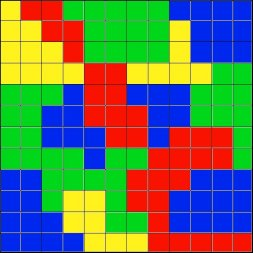
\includegraphics[width=4.452cm,height=4.452cm]{image/a2012Logique2eme-img026.jpg}
		\end{center}
		
		Résoudre les problèmes suivants~:

		\begin{enumerate}
			\item {
				vérifier si 2 pavés ($i_1$, $j_1$) et ($i_2$, $j_2$) 
				sont dans une même tache;}
			\item {
				trouver l'aire de la tache contenant le pavé ($i$, $j$);}
			\item {
				trouver le périmètre de la tache contenant le pavé ($i$, $j$);}
			\item {
				trouver l'aire de la plus grande tache du quadrillage;}
			\item {
				changer la couleur de la tache contenant le pavé ($i$, $j$) 
				avec une couleur entrée en paramètre.}
		\end{enumerate}
		
		Aide~: à partir d'un pavé de départ, on visitera les pavés 
		adjacents de même couleur, et on utilisera un tableau de
		booléens pour se rappeler si un pavé a déjà été traité.
	\end{Exercice}
	
	\begin{Exercice}{Les nombres de Catalan}
		Le \textit{n\textsuperscript{ième}} \textit{nombre de Catalan}, 
		noté $C_n$, correspond au nombre de différentes façons de 
		partager un polygone de \textit{n} + 2 côtés en triangles. 
		Par exemple $C_3=5$, car il y a 5 façons de partager un 
		pentagone en 3 triangles~:

		\begin{center}
		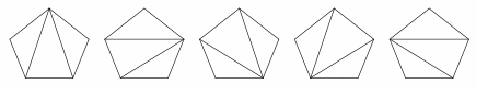
\includegraphics[width=12.659cm,height=2.387cm]{image/a2012Logique2eme-img027.png}
		\end{center}

		Trivialement, $C_0=1$, et on démontre que 
		$C_n=\overset{n-1}{\underset{i=0}{\sum }}C_i\ast C_{n-1-i}$

		\setcounter{saveenum}{\value{enumi}}
		\begin{enumerate}
			\item {
				Calculer les nombres de Catalan $C_i$ pour \textit{i} = 1, 2, 3, 4, 5. 
				Vérifiez que les valeurs obtenues correspondent bien à la 
				définition géométrique.}
			\item {
				Écrire l'algorithme récursif, issu directement de la formule 
				mathématique ci-dessus, permettant de calculer $C_n$. 
				Cette solution récursive vous semble-t-elle efficace ? 
				Combien d'appels récursifs sont exécutés pour le calcul 
				de $C_5$ ?}
		\end{enumerate}
	\end{Exercice}

